\section{Experimentacion Final}
Ahora, para concluir este trabajo, tomamos todos los algoritmos antes vistos y realizamos una experimentacion conjunta entre todos para mostrar como se comparan entre si.

La primera de las experimentaciones se realizará con grafos completos de 23 vertices con atistas elegidas al azar del 1 al 100. Sobre cada una de estas instancias se correrán todos los algoritmos antes descriptos, se tomarán cual es la mejor solucion encontrada por el mismo y cuanto tarda en encontrarla y en base a los resultados obtenidos se graficarán en una tabla comparativa donde puedan verse los resultados.

De esta experimentación, se obitiene que:

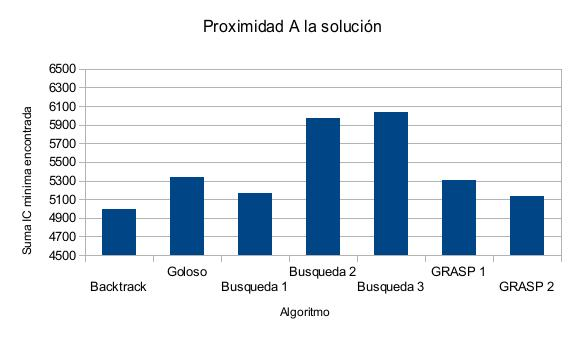
\includegraphics[scale=0.5]{Con/result.jpg}

Nuevamente puede observarse que las mejores heuristicas son las de busqueda local 1 y GRASP 2.

Y los tiempos obtenidos son:

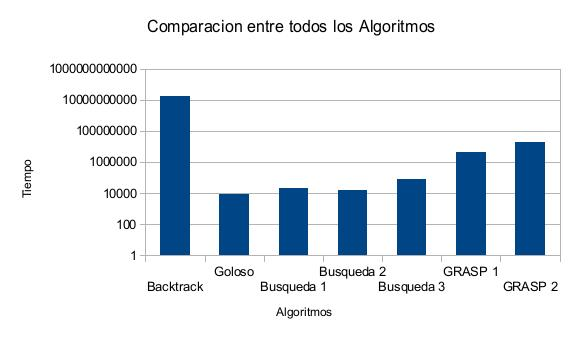
\includegraphics[scale=0.5]{Con/tiempos.jpg}

=========DECIR ALGO==============

\section{Conclución}
